
\documentclass{article}[14pt]
\usepackage{multicol, enumerate, enumitem, hyperref, color, soul, setspace, parskip, fancyhdr, amssymb, amsthm, amsmath, bbm, latexsym, units, mathtools}
\everymath{\displaystyle}
\usepackage[headsep=0.5cm,headheight=0cm, left=1 in,right= 1 in,top= 1 in,bottom= 1 in]{geometry}
\pagestyle{fancy}
\lhead{}
\chead{Answer Key for Module\,6\,-\,Polynomial\,Functions Version C}
\rhead{}
\lfoot{Summer\,C\,2020}
\cfoot{}
\rfoot{}
\begin{document}
\textbf{This key should allow you to understand why you choose the option you did (beyond just getting a question right or wrong). \href{https://xronos.clas.ufl.edu/mac1105spring2020/courseDescriptionAndMisc/Exams/LearningFromResults}{More instructions on how to use this key can be found here}.}

\textbf{If you have a suggestion to make the keys better, \href{https://forms.gle/CZkbZmPbC9XALEE88}{please fill out the short survey here}.}

\textit{Note: This key is auto-generated and may contain issues and/or errors. The keys are reviewed after each exam to ensure grading is done accurately. If there are issues (like duplicate options), they are noted in the offline gradebook. The keys are a work-in-progress to give students as many resources to improve as possible.}

\rule{\textwidth}{0.4pt}

26. Construct the lowest-degree polynomial given the zeros below. Then, choose the intervals that contain the coefficients of the polynomial in the form $x^3+bx^2+cx+d$.
$$ 4 + 3i \text{ and } 3 $$ 
The solution is $ x^{3} -11 x^{2} +49 x -75 $ 

\begin{enumerate}[label=\Alph*.] 
\item $ b \in [5, 19], c \in [48.59, 50.81], \text{ and } d \in [72.1, 78.9] $ 

 $x^{3} +11 x^{2} +49 x + 75$, which corresponds to multiplying out $(x-(4 + 3i))(x-(4 - 3i))(x + 3)$. 
\item $ b \in [-13, -10], c \in [48.59, 50.81], \text{ and } d \in [-77.1, -71.8] $ 

 * $x^{3} -11 x^{2} +49 x -75$, which is the correct option. 
\item $ b \in [-7, 3], c \in [-6.36, -5.71], \text{ and } d \in [6.8, 11.3] $ 

 $x^{3} + x^{2} -6 x + 9$, which corresponds to multiplying out $(x -3)(x -3)$. 
\item $ b \in [-7, 3], c \in [-7.02, -6.49], \text{ and } d \in [9.5, 14.3] $ 

 $x^{3} + x^{2} -7 x + 12$, which corresponds to multiplying out $(x -4)(x -3)$. 
\item $ \text{None of the above.} $ 

 This corresponds to making an unanticipated error or not understanding how to use nonreal complex numbers to create the lowest-degree polynomial. If you chose this and are not sure what you did wrong, please contact the coordinator for help. 
\end{enumerate} 
 
General Comments: Remember that the conjugate of $a+bi$ is $a-bi$. Since these zeros always come in pairs, we need to multiply out $(x-(4 + 3i))(x-(4 - 3i))(x-(3))$.

-----------------------------------------------

27. Describe the end behavior of the polynomial below.
$$ f(x) = -7(x + 2)^{3}(x - 2)^{8}(x - 7)^{2}(x + 7)^{3} $$ 

 
 The solution is  
 \begin{center} 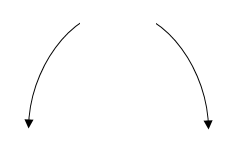
\includegraphics[width=0.3\textwidth]{../Figures/endBehaviorNegativeEvenC.png} \end{center}\begin{tabular}{|c|c|} 
\hline 
 & \tabularnewline 
 \textbf{A.} 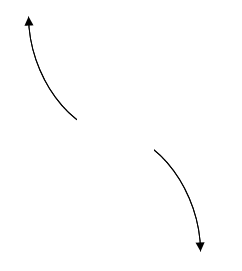
\includegraphics[width=0.3\textwidth]{../Figures/endBehaviorNegativeOddC.png} & \textbf{B.} 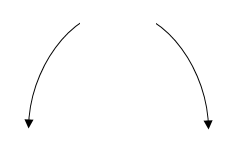
\includegraphics[width=0.3\textwidth]{../Figures/endBehaviorNegativeEvenC.png} \tabularnewline 
\hline 
 & \tabularnewline 
 \textbf{C.} 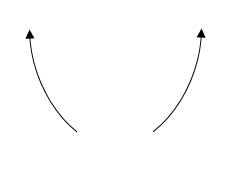
\includegraphics[width=0.3\textwidth]{../Figures/endBehaviorPositiveEvenC.png} & \textbf{D.} 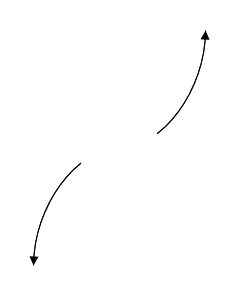
\includegraphics[width=0.3\textwidth]{../Figures/endBehaviorPositiveOddC.png} \tabularnewline 
\hline 
 E. None of the figures above. & \tabularnewline 
\hline 
 \end{tabular} 
 
\textbf{General Comments:} Remember that end behavior is determined by the leading coefficient AND whether the \textbf{sum} of the multiplicities is positive or negative.

-----------------------------------------------

28. Which of the following equations \textit{could} be of the graph presented below?
\begin{center} 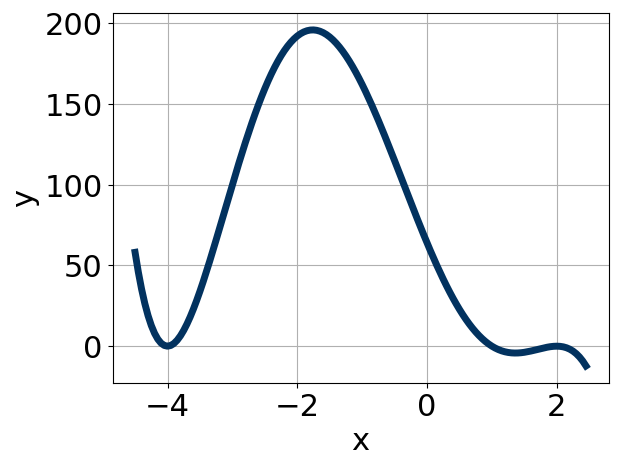
\includegraphics[width=0.3\textwidth]{../Figures/polyGraphToFunctionC.png} \end{center} 

The solution is $ -18(x + 4)^{10} (x - 2)^{6} (x - 1)^{5} $ 

\begin{enumerate}[label=\Alph*.] 
\item $ -18(x + 4)^{10} (x - 2)^{6} (x - 1)^{5} $ 

 * This is the correct option. 
\item $ -19(x + 4)^{8} (x - 2)^{7} (x - 1)^{7} $ 

 The factor $(x - 2)$ should have an even power. 
\item $ 6(x + 4)^{6} (x - 2)^{10} (x - 1)^{9} $ 

 This corresponds to the leading coefficient being the opposite value than it should be. 
\item $ -11(x + 4)^{6} (x - 2)^{7} (x - 1)^{4} $ 

 The factor $(x - 2)$ should have an even power and the factor $(x - 1)$ should have an odd power. 
\item $ 19(x + 4)^{10} (x - 2)^{6} (x - 1)^{4} $ 

 The factor $(x - 1)$ should have an odd power and the leading coefficient should be the opposite sign. 
\end{enumerate} 
 
General Comments: Draw the x-axis to determine which zeros are touching (and so have even multiplicity) or cross (and have odd multiplicity).

-----------------------------------------------

29. Construct the lowest-degree polynomial given the zeros below. Then, choose the intervals that contain the coefficients of the polynomial in the form $ax^3+bx^2+cx+d$.
$$ \frac{-3}{5}, \frac{-1}{4}, \text{ and } \frac{4}{5} $$ 
The solution is $ 100x^{3} +5 x^{2} -53 x -12 $ 

\begin{enumerate}[label=\Alph*.] 
\item $ a \in [98, 103], b \in [-167, -160], c \in [81, 89], \text{ and } d \in [-13, -10] $ 

 $100x^{3} -165 x^{2} +83 x -12$, which corresponds to multiplying out $(5x + 5)(4x + 4)(5x -5)$. 
\item $ a \in [98, 103], b \in [-1, 6], c \in [-56, -46], \text{ and } d \in [6, 15] $ 

 $100x^{3} +5 x^{2} -53 x + 12$, which corresponds to multiplying everything correctly except the constant term. 
\item $ a \in [98, 103], b \in [-15, -3], c \in [-56, -46], \text{ and } d \in [6, 15] $ 

 $100x^{3} -5 x^{2} -53 x + 12$, which corresponds to multiplying out $(5x -3)(4x -1)(5x + 4)$. 
\item $ a \in [98, 103], b \in [-118, -107], c \in [4, 17], \text{ and } d \in [6, 15] $ 

 $100x^{3} -115 x^{2} +13 x + 12$, which corresponds to multiplying out $(5x + 5)(4x -4)(5x -5)$. 
\item $ a \in [98, 103], b \in [-1, 6], c \in [-56, -46], \text{ and } d \in [-13, -10] $ 

 * $100x^{3} +5 x^{2} -53 x -12$, which is the correct option. 
\end{enumerate} 
 
General Comments: To construct the lowest-degree polynomial, you want to multiply out $(5x + 3)(4x + 1)(5x -4)$

-----------------------------------------------

30. Describe the zero behavior of the zero $x = -4$ of the polynomial below.
$$ f(x) = 3(x - 4)^{5}(x + 4)^{10}(x + 7)^{6}(x - 7)^{8} $$ 

 
 The solution is  
 \begin{center} 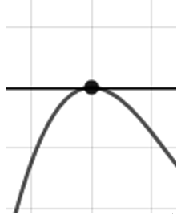
\includegraphics[width=0.3\textwidth]{../Figures/zeroBehaviorNegativeEvenC.png} \end{center}\begin{tabular}{|c|c|} 
\hline 
 & \tabularnewline 
 \textbf{A.} 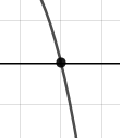
\includegraphics[width=0.3\textwidth]{../Figures/zeroBehaviorNegativeOddC.png} & \textbf{B.} 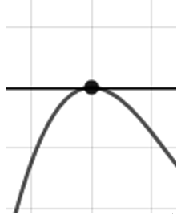
\includegraphics[width=0.3\textwidth]{../Figures/zeroBehaviorNegativeEvenC.png} \tabularnewline 
\hline 
 & \tabularnewline 
 \textbf{C.} 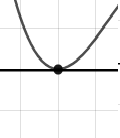
\includegraphics[width=0.3\textwidth]{../Figures/zeroBehaviorPositiveEvenC.png} & \textbf{D.} 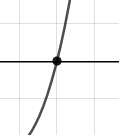
\includegraphics[width=0.3\textwidth]{../Figures/zeroBehaviorPositiveOddC.png} \tabularnewline 
\hline 
 E. None of the figures above. & \tabularnewline 
\hline 
 \end{tabular} 
 
\textbf{General Comments:} You will need to sketch the entire graph, then zoom in on the zero the question asks about.

-----------------------------------------------


\end{document}

